
%  \section{The analysis of FWHM behavior} 

Given that the observed seeing is by and large described by a single parameter, FWHM, 
we study three aspects of its variation, as follows.


\subsection{The FWHM dependence on wavelength} 

The Kolmogorov turbulence theory gives a standard formula for the FWHM of a long-exposure
seeing-limited PSF in a large telescope,
\begin{equation}
\textrm{FWHM}^{\rm Kolm}(\lambda, X) = \frac{0.976\lambda}{r_0(\lambda,X)}.
\label{eq:fwhmkolm}
\end{equation}
Here $\lambda$ is the wavelength, $X$ is the airmass, and $r_0$ is the Fried parameter.
We use $\lambda = 500$ nm as the reference wavelength,
\begin{equation}
r_0(\lambda,X) = r_0(500) \left(\frac{\lambda}{500}\right)^{1.2}
\frac{1}{X^{0.6}},
\label{eq:r0}
\end{equation}
where $r_0(500)$ is the $r_0$ for $\lambda=500$ nm and $X$=1, and $\lambda$ is 
expressed in nm.
Substituting Eq.~(\ref{eq:r0}) into (\ref{eq:fwhmkolm}), it is easy to see
\begin{equation}
\textrm{FWHM}^{\rm Kolm} \propto \lambda^{-0.2}.
\end{equation}


With the \vk~atmosphere model, the FWHM as in
Eq.~(\ref{eq:fwhmkolm}) needs an additional correction factor
which is a function of the outer scale $L_0$~\citep{Tokovinin2002},
\begin{equation}
\textrm{FWHM}^{\rm vonK}(\lambda, X) = \frac{0.976\lambda}{r_0(\lambda,X)}
\sqrt{1-2.183\left( \frac{r_0(\lambda,X) }{L_0} \right)^{0.356}}.
\end{equation}
If we still want to write FWHM$^{\rm vonK} \propto \lambda^{\alpha} $, 
$\alpha$ will be a function of $L_0$ and $r_0$ at a specified
wavelength and airmass, or equivalently, $L_0$ and FWHM$^{\rm vonK}$ at a
specified wavelength and airmass. Below, for FWHM, we will use FWHM$_r$,
PSF FWHM measurements from the 
$r$-band,
whose effective wavelength is 616.6 nm, and airmass of 1.

\begin{figure}
\centering
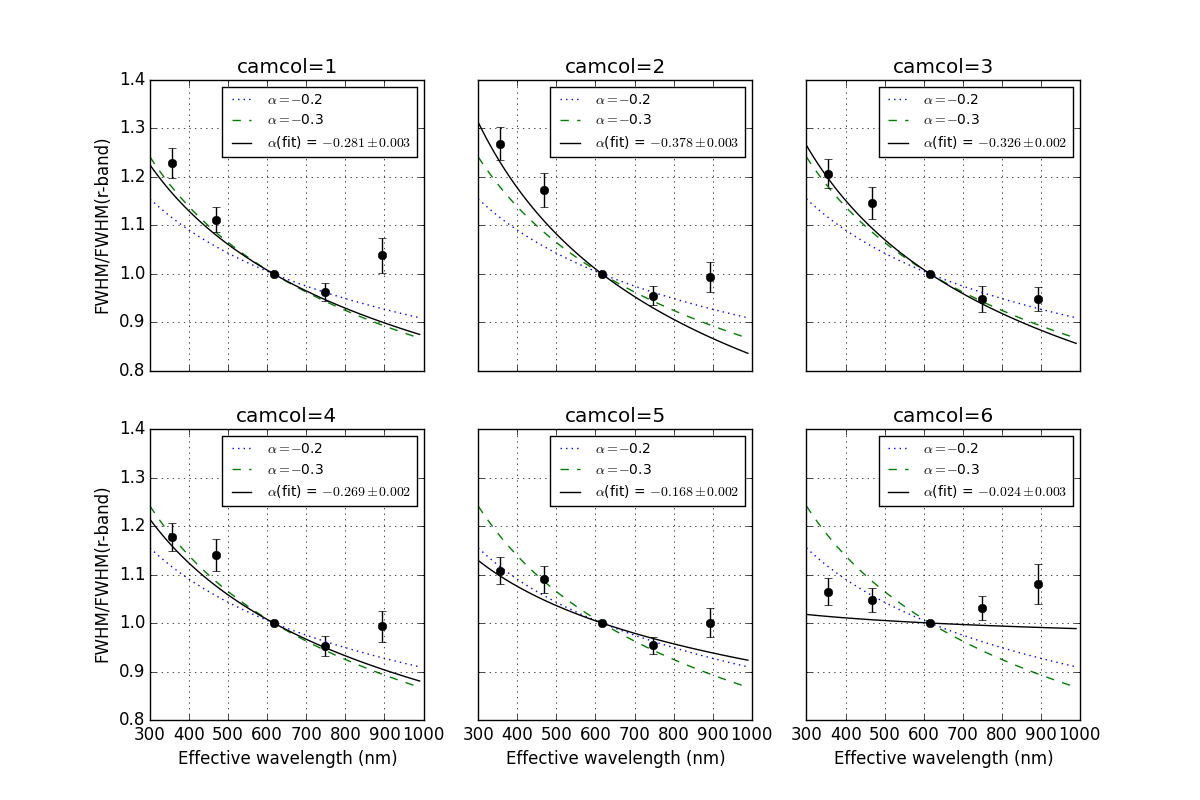
\includegraphics[width=0.9\textwidth]{FIGURES/fwhm_lambda.png}
\caption{FWHM as functions of wavelength for run 4874.
For comparison purposes, the $\alpha=-0.2$ (dotted) and $\alpha=-0.3$ (dashed) lines are
also shown.
\label{fig:fwhm_lambda}}
\end{figure}


\begin{figure}
\centering
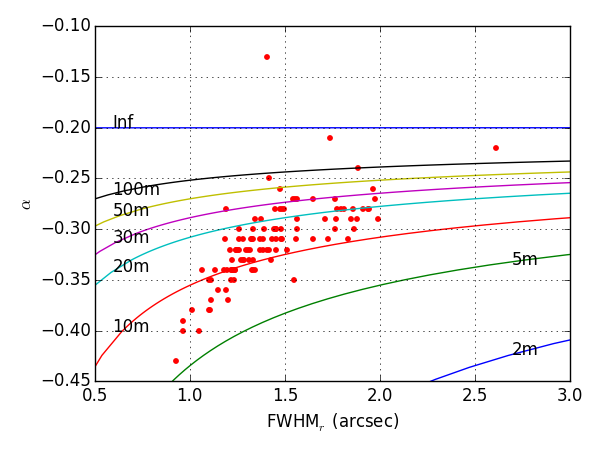
\includegraphics[width=0.5\textwidth]{FIGURES/alpha_fwhm.png}
\caption{The power-law index for the wavelength dependence of FWHM, $\alpha$, 
vs. the FWHM in the $r$-band for all the 108 Stripe 82 runs. 
The curves are predictions of the \vk~model, with $L_0$ ranging from 2 meters to infinity.
\label{fig:alpha_fwhm}}
\end{figure}

 
For each run from SDSS Stripe 82 data, and each camera column, we make
a least-square fit to
all the simultaneous FWHM measurements across the optical bands, to
estimate the power-law index $\alpha$.
All FWHM values are multiplied by $1/X^{0.6}$ to correct for the airmass effects.
We take into account that the same field number does not correspond to the same
time in all filters. The scanning order in the SDSS camera is $r$-$i$-$u$-$z$-$g$, with the delay between the two 
successive filters corresponding to 2 fields. That is, if we take the field number $F$ for the $r$-band, then
we need to take FWHM for the $i$-band from field $F-2$, for the $u$-band
from $F-4$, and so on. 

Fig.~\ref{fig:fwhm_lambda} shows such fits for run 4874. All FWHM are normalized using 
corresponding FWHM in the $r$-band taken at the same moment in time. Significant deviation 
from $\alpha = -0.2$, predicted by the Kolmogorov model, can be seen in most bands.


As discussed above, based on the \vk~atmosphere model, the
power $\alpha$ should be a function of outer scale $L_0$ and 
FWHM. 
Fig.~\ref{fig:alpha_fwhm} shows a scatter plot of $\alpha$ versus FWHM
in the $r$-band, for all the Stripe 82 runs.
A correlation between $\alpha$ and the FWHM seems to be present.
Similar correlations have been seen in Subaru images and reported by~\cite{subaruSeeing2016}.
The data points are overlaid with curves predicted by the 
\vk~model, with $L_0$ varying from 2 m to infinity.
The data clearly deviate from the Kolmogorov model prediction, which is
the horizontal line at $\alpha = -0.20$, with infinite $L_0$.
For example, for LSST's fiducial FWHM of 0.6 arcsec and the commonly assumed 
$L_0 = 30$ m, the \vk~model predicts an $\alpha$ value close to $-0.31$.



\subsection{Angular structure function} 

\begin{figure}
\centering
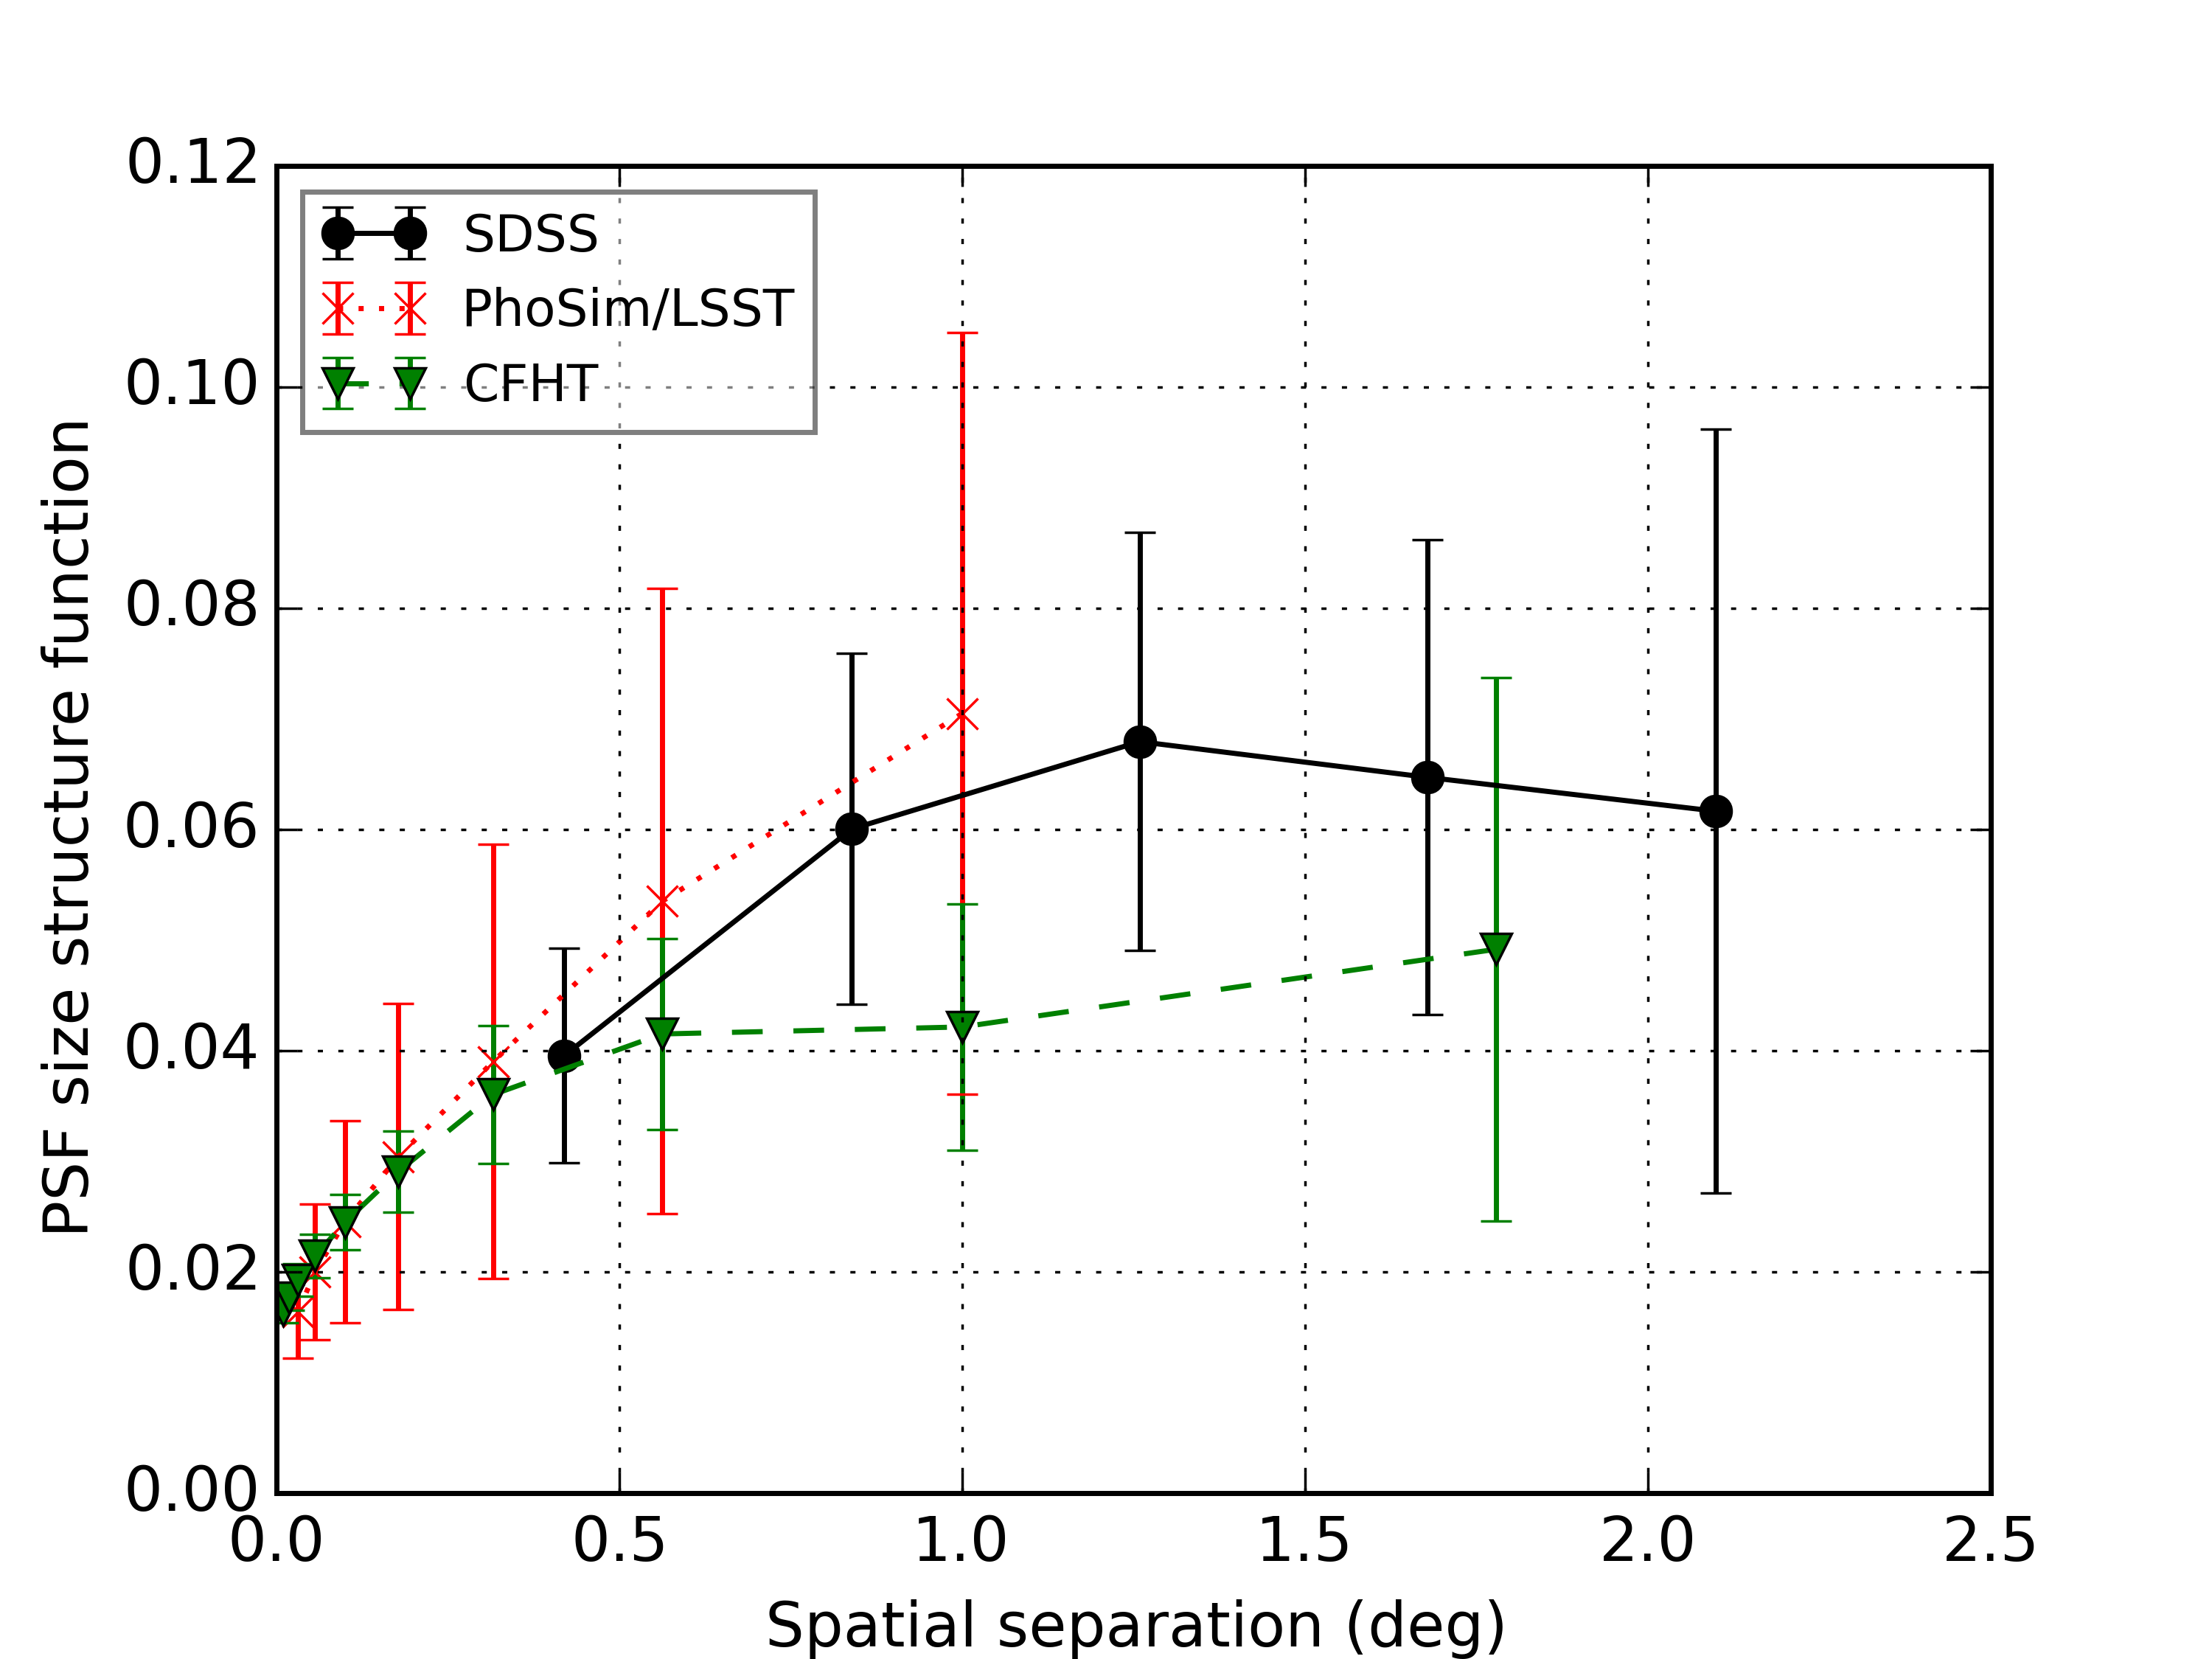
\includegraphics[width=0.5\textwidth]{FIGURES/spatial.png}
\caption{PSF size angular structure function using SDSS measurements
  combined over 86 out of the 108 runs with number of fields larger
  than 100, and comparisons with PhoSim simulations and CFHT
  measurements of the same quantity \citep{heymans2012}.
\label{fig:spatial}}
\end{figure}

To examine the spatial correlation of the FWHM, we compute the angular
structure function using PSF measurements from all 6 camera columns.
Our structure function is defined as
the root-mean-square of the PSF size differences of pairs of stars
in the same angular bin. 
The SDSS curves are combined for 86 out of the 108 Stripe 82 runs with the number of
fields larger than 100, and then combined for all
the bands. We also compared the structure functions for each band
separately, and found no statistically significant differences.
Results are shown in Fig.~\ref{fig:spatial}.

For comparison, Fig. ~\ref{fig:spatial} also shows the PSF angular
structure functions obtained using PhoSim~\citep{phosim} by simulating LSST,
and that from the CFHT PSF measurements~\citep{heymans2012}.
The PhoSim PSF profiles are obtained by simulating a grid of stars
spaced by 6 arcminutes with non-perturbed telescope and ideal sensors.
The results are averaged over 9 different atmosphere realizations with
different wind and screen parameters and airmass, and with 3 different
wavelength, 350 nm, 660 nm, and 970 nm.
The CFHT PSF size measurements were made in the $i$-band, and provided
by the authors of~\cite{heymans2012}.
The 3 curves in Fig.~\ref{fig:spatial} appear to be quantitatively
consistent with each other, even though they are for telescopes at
different sites and with different optics.
The structure function is seen to start saturating at a separation of
$\sim 0.5 - 1.0$ degree, where the PSF size typically differ on the
scale of $\sim 0.05$ arcsec.

\subsection{Temporal auto-correlation function}

To study the temporal behavior of the seeing, we look at its
 power spectrum.
Fig.~\ref{fig:psd} shows the temporal power spectral density (PSD) of the
PSF FWHM for 6 camera columns, in run 4874, $r$-band.
The time difference between subsequent fields is 36 seconds.
We fit the PSD using two competing models.
The first is a damped random walk (DRW) model~\citep{zeljkoBook},
\begin{equation}
\textrm{PSD}(f) = \frac{\tau^2 SF^2_{\infty}}{1+(2\pi f \tau)^2},
\end{equation}
where $f$ is the temporal frequency, $SF_{\infty}$ is the asymptotic
value of the structure function, and $\tau$ is the
characteristic timescale.
The solid curves in Fig.~\ref{fig:psd} show fits using this model.
Note that due to the lack of data toward the low-frequency end, the
first and second bins are four and two times wider than the
rest of the bins, respectively.
Combining fit results for all camera columns and optical bands for run 4874
gives $\tau = 23.6 \pm 1.3$ minutes.
Making the same fits for all the 108 runs in Stripe 82, 
we obtain the $\tau$ distribution vs. the duration of each
run, as shown in Fig.~\ref{fig:hist} (left).
The shorter runs tend to give smaller timescale, due to the lack of
data toward the low-frequency end of the spectra.
% therefore are unable to
% constrain the location of the "knee" during the fit. They tend to
% push the "knee" to the right.
There are a total of 12 runs longer than 6 hours.
Their characteristic timescale is general within the range of
$\sim15-25$ minutes.
This is generally consistent with ~\cite{Racine1996}, where a timescale of 
$\tau = 17 \pm 1$ minutes was found.

The temporal PSD of the FWHM can also be well-fitted using a power
law,
\begin{equation}
\textrm{PSD}(f) = B f^\beta,
\end{equation}
where $B$ is the normalization factor, and $\beta$ is the power-law
index.
Fits to data in run 4874, $r$-band are shown in
Fig.~\ref{fig:psd} as dashed lines.
Combining fit results for all camera columns and optical bands for run 4874
gives $\beta = -1.29\pm 0.09$.
Making the same fits for all the 108 runs in Stripe 82, 
we obtained the $\beta$ distribution vs. the duration each
run, as shown in Fig.~\ref{fig:hist} (right).
The shorter runs give $\beta$ values with a larger variance.
Most of the longer runs have power-law index roughly between $-1.5$ and $-1.0$.

The power law fit systematically over predicts the low-frequency part of the PSD,
while $1/f^2$ high-frequency behavior of the DRW model is too steep. One could argue that
some hybrid model would work, but that's beyond the scope of our work. 

\begin{figure}
\centering
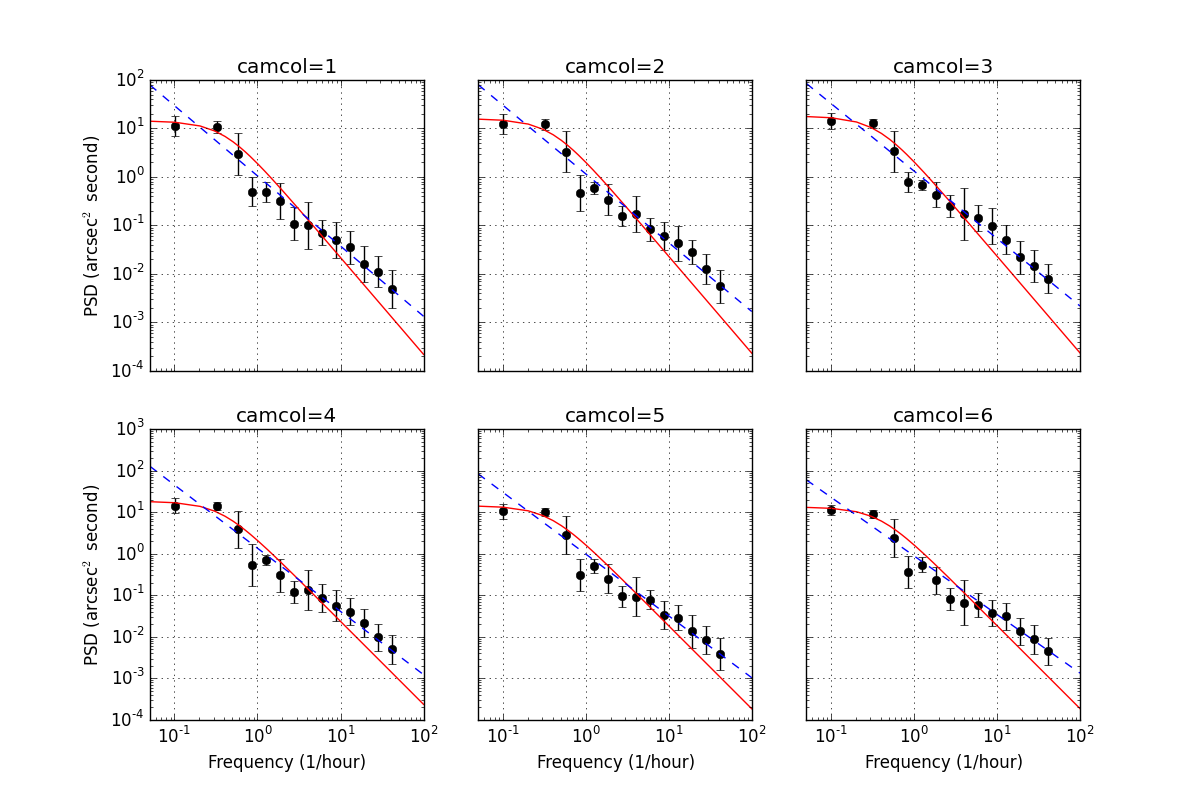
\includegraphics[width=0.9\textwidth]{FIGURES/temporalPSD.png}
\caption{PSF size temporal power spectral density for run 4874, r-band. 
The solid lines are fits using the damped random walk model. 
The dashed lines show fits to the power-law model.
\label{fig:psd}}
\end{figure}

\begin{figure}
\centering
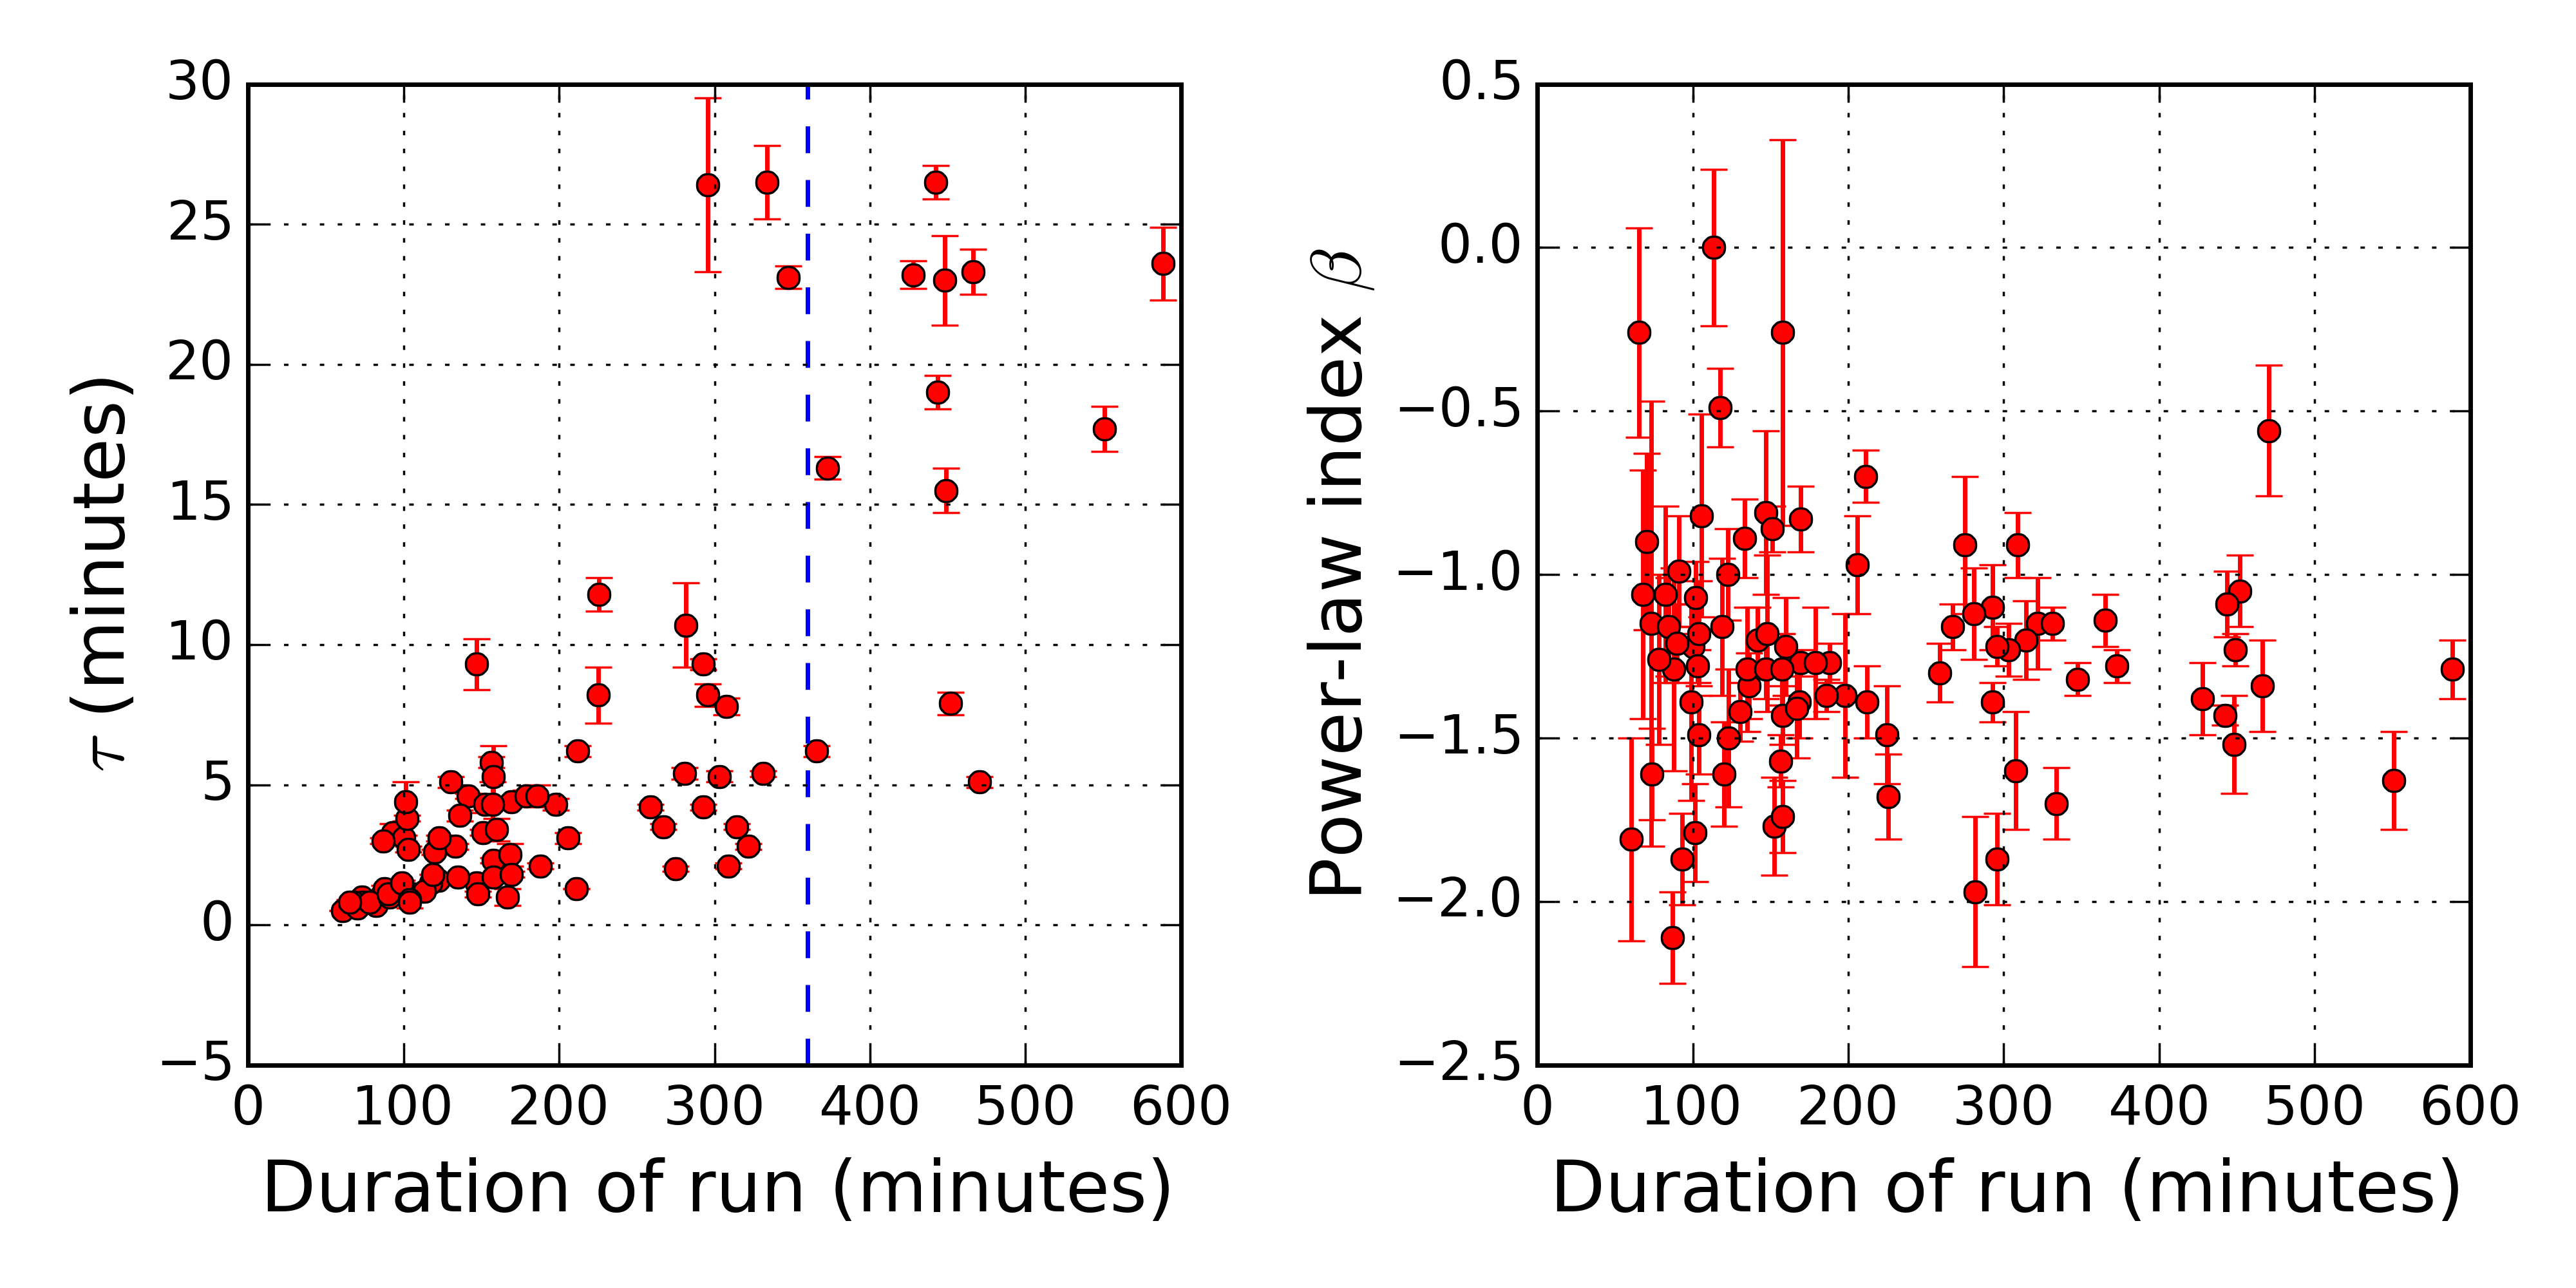
\includegraphics[width=0.9\textwidth]{FIGURES/taubeta.png}
\caption{Left: The damped random walk characteristic
  timescale $\tau$ for all 108 runs in Stripe 82 vs. the duration of 
each run. Right: The power-law index $\beta$ for all 108 runs vs. the
duration of each run.
\label{fig:hist}}
\end{figure}


Following~\cite{Racine1996}, we also define the structure-function-like quantity
\begin{equation}
       f(\Delta t) = {| \theta(t+\Delta t) - \theta(t)| \over  \theta(t+\Delta t) + \theta(t) },
\end{equation} 
where $\theta$ is seeing.
We then fit the mean value of $f(\Delta t)$ to 
\begin{equation}
    < f(\Delta t) > =  f(\Delta t) ^\infty \, \left[ 1 - \exp(-\Delta
      t/\tau)^\gamma \right],
\label{eq:fdt}
\end{equation} 
with $f(\Delta t) ^\infty$, $\tau$ and $\gamma$ as free parameters.
The timescale $\tau$ is found to be mostly within the range of 15 to
25 minutes, and $\gamma$ between 1.0 and 1.5.
Fig.~\ref{fig:fdt} (left) shows one example of such fits.
The distribution of $\tau$ vs. the duration of each
run is shown in Fig.~\ref{fig:fdt} (right). The runs shorter than 20
minutes are obviously not good for measuring the timescale. We have
set $\tau$ to zero for those runs.
Still, the short runs have larger variances in $\tau$.
If we look at only those runs longer than 6 hours,
the timescale $\tau$ is mostly between 15 and 25 minutes.

\begin{figure}
\centering
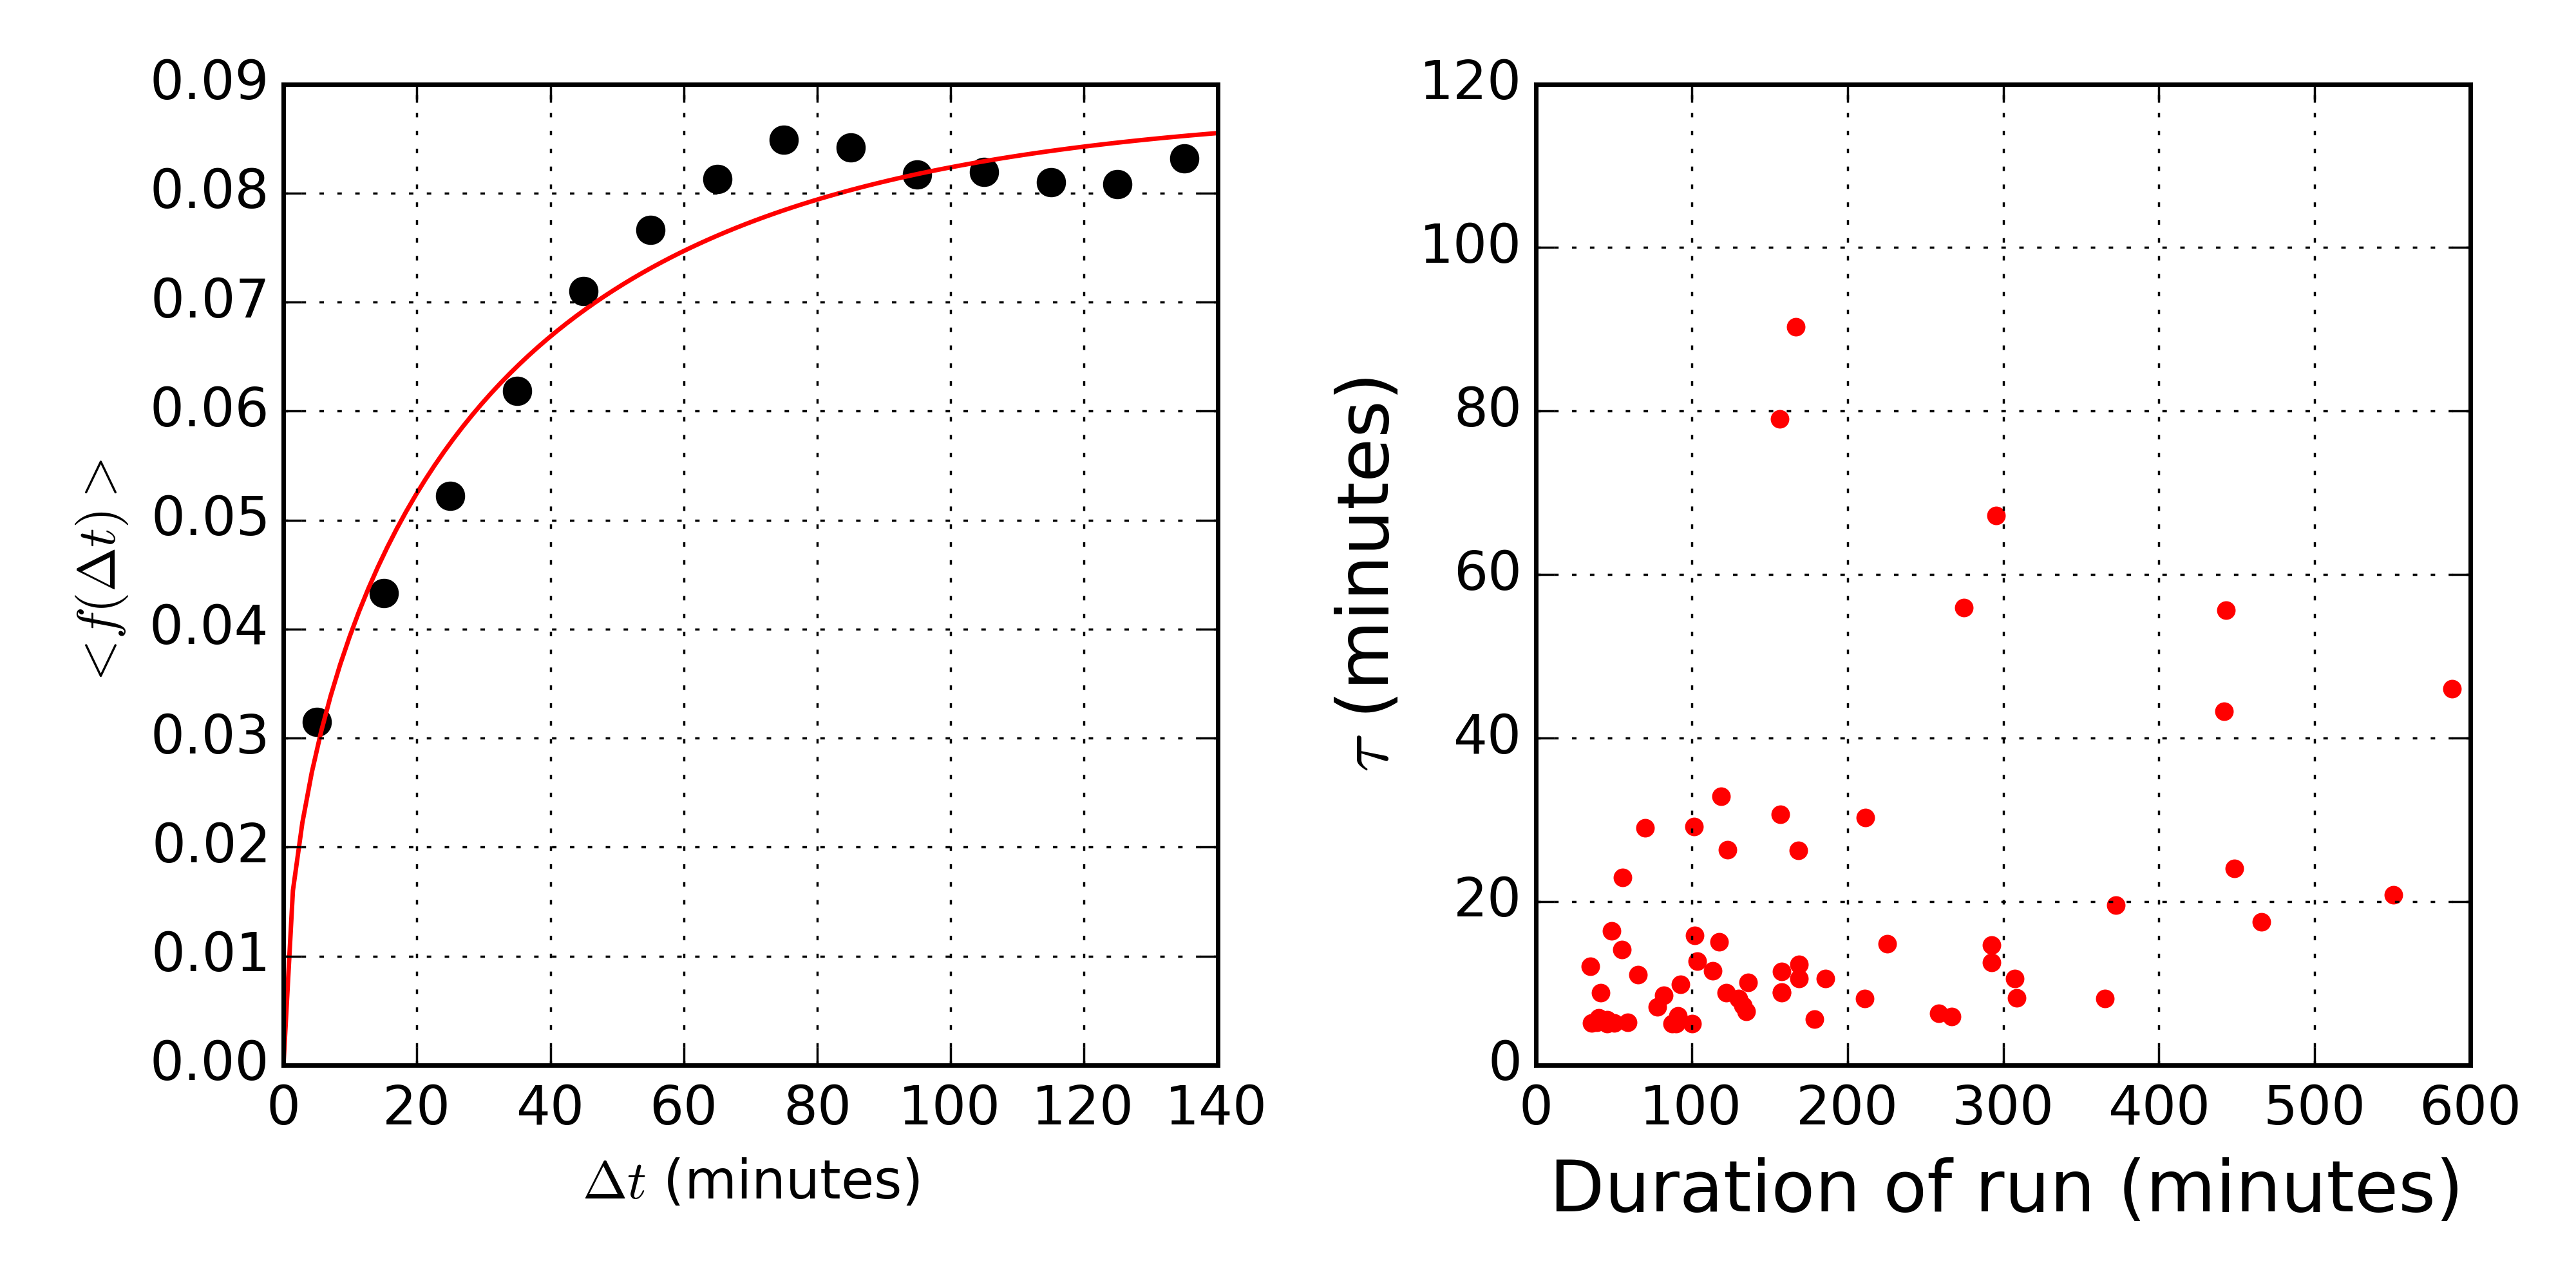
\includegraphics[width=0.9\textwidth]{FIGURES/fdt.png}
\caption{Left: The average normalized seeing difference, $<f(\Delta t)>$, as
  a function of the time separation, $\Delta t$, for run 4874, camera
  column 1, in the $r$-band.
The fit to Eq.~(\ref{eq:fdt}) gives $\tau = 25.9$ minutes and $\gamma$
= 1.49.
Right: The timescale $\tau$ for all 108 runs vs. the duration of each run.
\label{fig:fdt}}
\end{figure}
